\documentclass[a4paper,10pt]{article}

%A Few Useful Packages
\usepackage{marvosym}
\usepackage{fontspec} 					%for loading fonts
\usepackage{xunicode,xltxtra,url,parskip} 	%other packages for formatting
\RequirePackage{color,graphicx}
\usepackage[usenames,dvipsnames]{xcolor}
\usepackage[big]{layaureo} 				%better formatting of the A4 page
% an alternative to Layaureo can be ** \usepackage{fullpage} **
\usepackage{supertabular} 				%for Grades
\usepackage{titlesec}					%custom \section

%Setup hyperref package, and colours for links
\usepackage{hyperref}
\definecolor{linkcolour}{rgb}{0,0.2,0.6}
\hypersetup{colorlinks,breaklinks,urlcolor=linkcolour, linkcolor=linkcolour}

\renewcommand{\familydefault}{\rmdefault} 


\titleformat{\section}{\Large\scshape\raggedright}{}{0em}{}[]
\titlespacing{\section}{0pt}{3pt}{3pt}
%Tweak a bit the top margin
%\addtolength{\voffset}{-1.3cm}

%Italian hyphenation for the word: ''corporations''
\hyphenation{im-pre-se}

\usepackage[absolute]{textpos}
\usepackage{graphicx}
\usepackage{wrapfig}

\usepackage{changepage}

\usepackage{enumitem}
\usepackage{booktabs}

\setlength{\TPHorizModule}{30mm}
\setlength{\TPVertModule}{\TPHorizModule}
\textblockorigin{2mm}{0.65\paperheight}
\setlength{\parindent}{0pt}

%--------------------BEGIN DOCUMENT----------------------
\begin{document}

\pagestyle{empty} % non-numbered pages

\font\fb=''[cmr10]'' %for use with \LaTeX command

%--------------------TITLE-------------


%\begin{wrapfigure}{l}{0.19\textwidth}
    %\centering
%    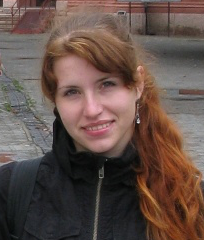
\includegraphics[width=0.19\textwidth]{photo}
%\end{wrapfigure}

%--------------------SECTIONS-----------------------------------
%Section: Personal Data

%\begin{figure}[ht!]
%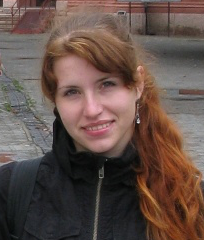
\includegraphics[width=0.25\textwidth]{photo.png}
%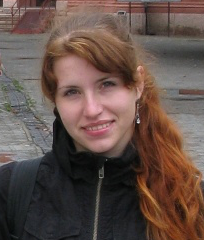
\includegraphics[width=71.967mm]{photo.png}
%\end{figure}
%\photo[64pt][0.4pt]{IMG_784510}
%\section{Personal Data}


\begin{minipage}{.67\textwidth}

%\raggedright

\par{{\Huge \textsc{Natalia Tymchuk}
	}\bigskip\par}

\vspace{2ex}

\begin{adjustwidth}{-2mm}{}

\begin{tabular}{l l}
%\hspace{-2mm}	
	\multicolumn{2}{l}{\textbf{Personal Information}} \\
	\textsc{Nationality:} & \hspace{-2mm}Ukrainian\\
	\textsc{Born:} & \hspace{-2mm}9.02.1991\\
	\\
	\multicolumn{2}{l}{\textbf{Contacts}} \\
   \textsc{Address:}   & \hspace{-2mm}Via G. Buffi 13, 6904, \\
   						& \hspace{-2mm}Lugano, Switzerland \\
    \textsc{email:}     & \hspace{-2mm}\href{mailto:natalia.tymchuk@usi.ch}{natalia.tymchuk@usi.ch}
\end{tabular}
\end{adjustwidth}
\end{minipage}%
\begin{minipage}{4cm}
  \vspace{15mm}\hspace{9mm}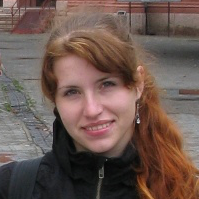
\includegraphics[width=3cm]{photoCV}
\end{minipage}

%\begin{minipage}{.2\textwidth}
%  \raggedleft
%  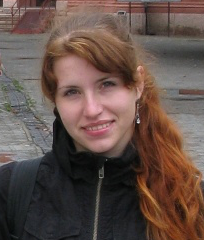
\includegraphics[width=2.5cm]{photo}
%\end{minipage}%



%TABLE
%\begin{table}[h!]
%     \begin{center}
%     \begin{tabular}{ p{3cm}  p{5cm} c }
%		\textbf{Personal}			& \textbf{Information}	& \raisebox{-\totalheight}{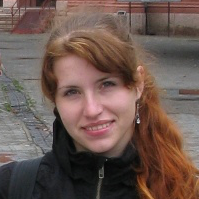
\includegraphics[width=0.2\textwidth, height=35mm]{photoCV.png}} 
%\\ 
%		\textsc{Nationality:} 	& Ukrainian &\\
%		\textsc{Born:} 			& 9.02.1991 &\\
%       \textbf{Contacts} 		& &\\
%		\textsc{Address:}   		& Via G. Buffi 13, 6904, & \\
									%& Lugano, Switzerland 
 		%\textsc{email:}     		& \href{mailto:natalia.tymchuk@usi.ch}{natalia.tymchuk@usi.ch}     
      %&\raisebox{-\totalheight}{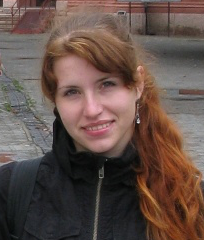
\includegraphics[width=0.2\textwidth, height=35mm]{photo.png}}      
%      \end{tabular}
%      \end{center}
%      \end{table}

%TABLE
\vspace{1ex}


%Section: Education
\section{Education}
\begin{adjustwidth}{-2mm}{}
 \begin{tabular}{p{2cm} p{11cm}}	

 \textsc 2015 -- now  & \textbf{Ph.D. in  \textsc{Informatics}}\\
 &Universita della Svizzera Italiana, Lugano, Switzerland.\\ 
 &Advisor: Prof. Dr. Michele Lanza\\
\\
 \textsc 2012 -- 2013 &  \textbf{Master of Science in \textsc{Mathematics}}\\ 
& Ivan Franko National University of Lviv, Ukraine.\\
  & Master's project: ``Properties of loxodromic function"| \small Advisor: Prof. Dr. Andriy \textsc{Kondratyk}\\
& I got the diploma with honours.\\
 \\
 \textsc 2008 -- 2012 & \textbf{Bachelor of Science in \textsc{Mathematics}}\\ 
 &Ivan Franko National University of Lviv, Ukraine.\\
 & Bachelor's project: ``Loxodromic functions"| \small Advisor: Prof. Dr. Andriy \textsc{Kondratyk}\\
 & Course work: ``Convex functions"| \small Advisor: Prof. Dr. Andriy \textsc{Kondratyk}\\
  \\
\textsc 2004 --  2008 & \textbf{Highschool diploma}\\
&Lviv Physics and Mathematics Lyceum\\
&Specialization in Physics and Mathematics\\  
\end{tabular}
\end{adjustwidth}

%Section:  Experience 
\section{Experience and Projects}
\begin{adjustwidth}{-2mm}{}
\begin{tabular}{p{2cm} p{11cm}}
 \textsc{Mar-Sep} & Project: \textbf{Voronyj diagram builder for Roassal}\\ 
\hspace{8mm}{2014}&Responsibilities: development of Voronyj (Voronoi) diagram builder in Pharo (Smalltalk dialect), using Roassal (agile visualisation engine).\\
&\footnotesize{You can read more here:  \href{http://natalia.tymchuk.me/RTVoronyjDiagram/}{natalia.tymchuk.me/RTVoronyjDiagram/} }\\
&This project won first place in Second Visualization Contest with Roassal.\\\multicolumn{2}{c}{} \\

 \textsc{May-Oct} & Project: \textbf{ODE solver for SciSmalltalk}\\
  \hspace{9mm}{2013}&\emph{Google Summer of Code (mentored by ESUG)}\\
 &Responsibilities: development ODE (Ordinary Differential Equations) solver for SciSmalltalk project in Pharo (Smalltalk dialect).\\
&\footnotesize{ You can read more about this project here: \href{http://gsoc2013.esug.org/projects/scismalltalk}{gsoc2013.esug.org/projects/scismalltalk}  or you can read more about what I did on my blog: \href{http://blog.natalia.tymchuk.me}{blog.natalia.tymchuk.me}.}\\\multicolumn{2}{c}{} \\

\end{tabular}
\end{adjustwidth}

%Section: MOOC
\section{Massive Open Online Courses}
\begin{adjustwidth}{-2mm}{}
\begin{tabular}{p{2cm} p{11cm}}
\textsc{2013} & \textbf{An Introduction to Interactive Programming in Python}\\
  &Coursera � Rice University. \footnotesize{Completion Score: 96.4/100}\\
  &\footnotesize{ \href{http://natalia.tymchuk.me/Coursera%20interactivepython%202014.pdf}{See certificat} }\\
  \\
 \textsc{2012} & \textbf{Learn to Program: The Fundamentals} \\ 
 &Coursera � University of Toronto. \footnotesize{Completion Score: 98,2/100}\\
 &\footnotesize{\href{http://natalia.tymchuk.me/Coursera%20programming1%202014.pdf}{See certificat }}\\  
\end{tabular}
\end{adjustwidth}


%Section: Languages
\section{Languages}
\begin{adjustwidth}{-2mm}{}
\begin{tabular}{p{2cm} p{11cm}}
 \textsc{Ukrainian:}&Mothertongue\\
\textsc{English:}&Upper Intermediate\\
\end{tabular}
\end{adjustwidth}


%\newpage
%\hypertarget{gmat}{\textsc{Gmat}\setmainfont{LMRoman10 Regular}\textregistered\setmainfont[SmallCapsFont=Fontin-SmallCaps]{Fontin-Regular}}

%\XeTeXpdffile ''GMAT.pdf'' page 1 scaled 800

\end{document}
